\chapter{Gráficos do Experimento 5}

\begin{figure}[H]
\centering

\includegraphics[scale=1]{apxe/agco1/1}

\end{figure}

\begin{figure}[H]
\centering

\includegraphics[scale=1]{apxe/agco1/2}

\end{figure}

\begin{figure}[H]
\centering

\includegraphics[scale=1]{apxe/agco1/3}

\end{figure}
\begin{figure}[H]
\centering

\includegraphics[scale=1]{apxe/agco1/4}

\end{figure}
\begin{figure}[H]
\centering

\includegraphics[scale=1]{apxe/agco1/5}

\end{figure}
\begin{figure}[H]
\centering

\includegraphics[scale=1]{apxe/agco1/6}

\end{figure}
\begin{figure}[H]
\centering

\includegraphics[scale=1]{apxe/agco1/7}

\end{figure}
\begin{figure}[H]
\centering

\includegraphics[scale=1]{apxe/agco1/8}

\end{figure}
\begin{figure}[H]
\centering

\includegraphics[scale=1]{apxe/agco1/9}

\end{figure}
\begin{figure}[H]
\centering

\includegraphics[scale=1]{apxe/agco1/10}

\end{figure}


\begin{figure}[H]
\centering

\includegraphics[scale=1]{apxe/agco2/1}

\end{figure}

\begin{figure}[H]
\centering

\includegraphics[scale=1]{apxe/agco2/2}

\end{figure}

\begin{figure}[H]
\centering

\includegraphics[scale=1]{apxe/agco2/3}

\end{figure}

\begin{figure}[H]
\centering

\includegraphics[scale=1]{apxe/agco2/4}

\end{figure}

\begin{figure}[H]
\centering

\includegraphics[scale=1]{apxe/agco2/5}

\end{figure}

\begin{figure}[H]
\centering

\includegraphics[scale=1]{apxe/agco2/6}

\end{figure}

\begin{figure}[H]
\centering

\includegraphics[scale=1]{apxe/agco2/7}

\end{figure}

\begin{figure}[H]
\centering

\includegraphics[scale=1]{apxe/agco2/8}

\end{figure}

\begin{figure}[H]
\centering

\includegraphics[scale=1]{apxe/agco2/9}

\end{figure}

\begin{figure}[H]
\centering

\includegraphics[scale=1]{apxe/agco2/10}

\end{figure}


\end{document}